\documentclass[12pt]{article}

\usepackage[letterpaper,margin=1in]{geometry}

\setlength{\parindent}{0pt}

\usepackage{amssymb}
\usepackage{amsmath}

\usepackage{multicol}

\usepackage{tikz}

\newcommand{\headerText}{
  MA 126-103 | Summer 2017 | Dr. Clontz
}

\usepackage{fancyhdr}
\pagestyle{fancy}
\renewcommand{\headrulewidth}{0pt}% Default \headrulewidth is 0.4pt
\renewcommand{\footrulewidth}{0pt}% Default \footrulewidth is 0pt
\chead{\footnotesize\bf\headerText}
\cfoot{}

\newcommand{\csch}{\operatorname{csch}}
\newcommand{\sech}{\operatorname{sech}}





\begin{document}


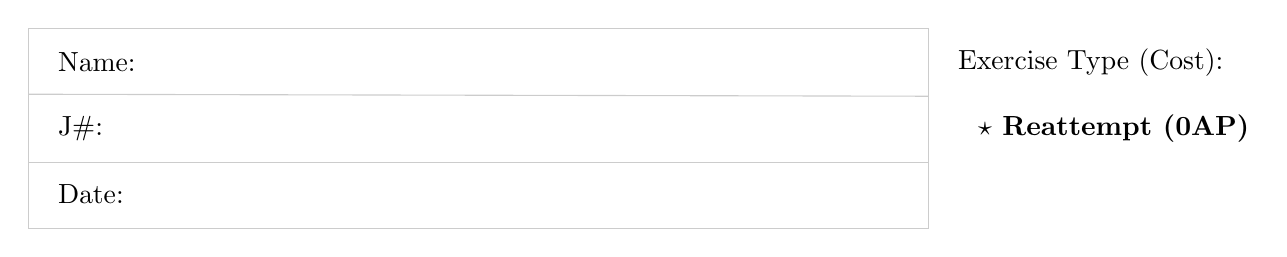
\begin{tikzpicture}[x=1in,y=1in]
  \draw[color=black!20] (0,0) rectangle (4.5,1);
  \draw[color=black!20] (0,0.67) -- (4.5,0.66);
  \draw[color=black!20] (0,0.33) -- (4.5,0.33);

  \node[anchor=west] at (0.1,0.83) {Name:};
  \node[anchor=west] at (0.1,0.5) {J\#:};
  \node[anchor=west] at (0.1,0.17) {Date:};

  \node[anchor=west] at (4.6,0.83) {Exercise Type (Cost):};
  \node[anchor=west] at (4.7,0.5) {\textbf{\(\star\) Reattempt (0AP)}};
\end{tikzpicture}

\vspace{1em}

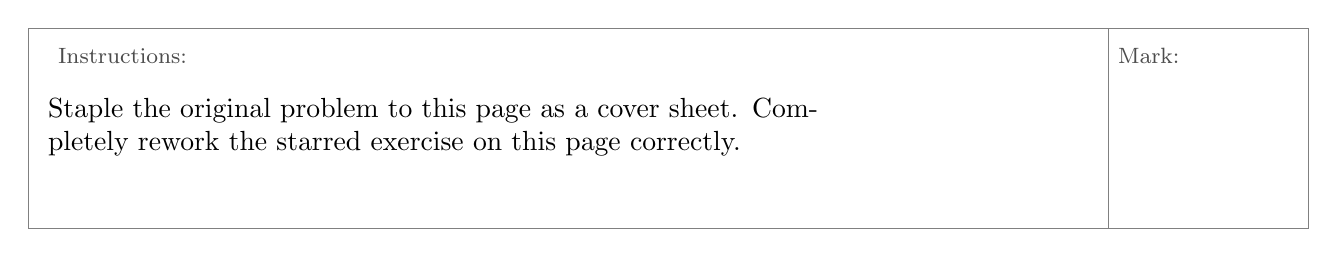
\begin{tikzpicture}[x=1in,y=1in]
  \draw[color=black!50] (0,0) rectangle (6.4,1);
  \draw[color=black!50] (5.4,0) -- (5.4,1);
  % \draw[dashed,color=black!20] (5.4,0.25) -- (6.4,0.25);

  \node[anchor=north west,text width=4in,color=black!70] at (0.1,0.95) {\footnotesize Instructions:};
  \node[anchor=north west,text width=4in] at (0.05,0.7) {Staple the original problem to this page as a cover sheet. Completely rework the starred exercise on this page correctly.};

  \node[anchor=north west,color=black!70] at (5.4,0.95) {\footnotesize Mark:};
  % \node[anchor=south east,color=black!70] at (5.4,0) {\footnotesize \(\star\) reattempt due on:};
\end{tikzpicture}

\vspace{1em}

\end{document}
